\chapter{INTRODUCTION}\
\pagenumbering{arabic}
\hspace*{0.3in}Today man is able to send and receive any form 
of data may be an e-mail or an audio or video 
just by the click of a button but did he ever 
think how securely his data id being transmitted 
or sent to the other person safely without any 
leakage of information?? The answer lies in 
cyber security. Today Internet is the fastest 
growing infrastructure in every day life. In 
today’s technical environment many latest 
technologies are changing the face of the man 
kind. But due to these emerging technologies 
we are unable to safeguard our private 
information in a very effective way and hence 
these days cyber crimes are increasing day by 
day. Today more than 60 percent of total 
commercial transactions are done online, so this 
field required a high quality of security for 
transparent and best transactions. Hence cyber 
security has become a latest issue. The scope of 
cyber security is not just limited to securing the 
information in IT industry but also to various 
other fields like cyber space etc.
\\

\hspace*{0.3in}Today, almost everybody in the world uses social media
but most of them do not always give concern to security. This
is the procedure of analysis of social media dynamic data to
save from ultimatum in business. Every industry has to face
some sort of a special collection of risks on social. Many put
themselves at the center of controversy or in the press of the
organization. In the present, many people are using social
media in a high percentage. They did not consider their data
and information security. In the present time, Social media
networks are always the main priority target of cyber security
attacks. Because of their massive user base. There are many
studies that explore vulnerabilities of security as well as issues
of privacy in social networking sites. Those researches made
better recommendations to diminish from security risks.
Therefore this analysis focuses mainly on factors of study
impact among users of public sector organizations for the
protection of social media emphasis. Particularly in the
education sector.\\
\hspace*{0.3in}In current times many people are using social media.
Every social media application asking personal details for
signup. Every people give their all details depends with their
privacy without considering whether they are using is more
secure or less secure. Here is the breakdown of personal
information that all social media platforms are gained by
users. Name, email, address book, credit card information,
debit card information, language, etc. There are couple of
tools in security tools. They are social media developers
realized security tools and external web services realized
tools. The combination of those two tools allow for a user to
complete the security of accounts. There are some of them as
an example; two-factor authentication, private account,
security checkup, login notification, password strength
Hiruni Fernando
Department of Information Technology
Sri Lanka Institute of Information Technology
Malabe, Sri Lanka
fernandohiruni55@gmail.com
Shashipraba Perera
Department of Information Technology
Sri Lanka Institute of Information Technology
Malabe, Sri Lanka
shashipraba.56@gmail.com
2
checker, trusted contacts, periodic password changes, external
application or site access checkup, email breaches checkup,
identification code etc\\
\begin{figure}
    \centering
    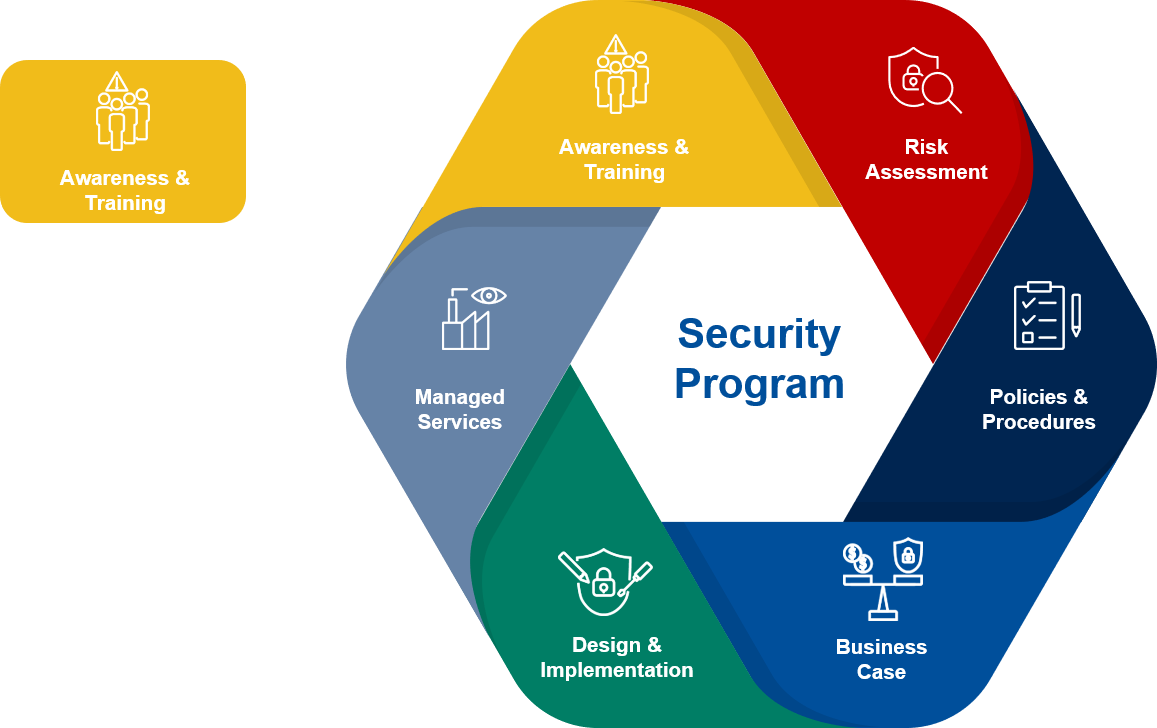
\includegraphics[width=1\linewidth]{AT.png}
    \caption{Security Program}
    \label{fig:enter-label}
\end{figure}
\hspace*{0.3in}Even the latest technologies like cloud 
computing, mobile computing, E-commerce, net 
banking etc also needs high level of security. 
Since these technologies hold some important 
information regarding a person their security 
has become a must thing. Enhancing cyber
security and protecting critical information 
infrastructures are essential to each nation's 
security and economic wellbeing. Making the 
Internet safer (and protecting Internet users) has 
become integral to the development of new 
services as well as governmental policy. The 
fight against cyber crime needs a 
comprehensive and a safer approach. Given that 
technical measures alone cannot prevent any 
crime, it is critical that law enforcement 
agencies are allowed to investigate and 
prosecute cyber crime effectively. Today many 
nations and governments are imposing strict 
laws on cyber securities in order to prevent the 
loss of some important information. Every 
individual must also be trained on this cyber 
security and save themselves from these 
increasing cyber crimes. \\